\clearpage\subsection{Horizontal Reflections}
A horizontal reflection is achieved when $b$ is negative. A negative value for $b$ means every input for a function $f(x)$ that used to be positive becomes negative. For example, when $b = 1$ for the function $f(x) = \dfrac{1}{x}$, inputting $x = 1$ produces $y = 1$. However, for a function $g(x) = \dfrac{1}{-x}$, where $b = -1$, plugging $x = 1$ produces $y = -1$.
\begin{center}\vspace{-0.25cm}
    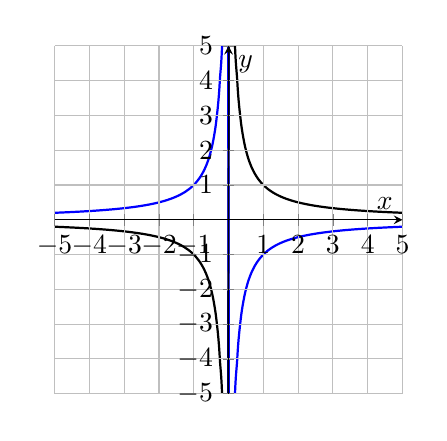
\begin{tikzpicture}
        \begin{axis} [
            axis lines=middle,
            xlabel = $x$, ylabel = {$y$},
            xmin = -5, xmax = 5,
            ymin = -5, ymax = 5,
            xtick distance={1}, ytick distance={1},
            grid = both,
            width = 6cm,
            height = 6cm,
            smooth,
            axis on top
        ]

            \addplot[black, thick, smooth, domain = -5:5, samples = 100]{1 / x};
            \addplot[blue, thick, smooth, domain = -5:5, samples = 100]{1 / (-1 * x)};
        \end{axis}
    \end{tikzpicture}\\
    $f(x) = \dfrac{1}{x}$ (Black), 
    $f(x) = \dfrac{1}{-x}$ (Blue),
\end{center}

\begin{definition}
    Given a function $f(x)$, a vertical reflection, also called a reflection along the $y$-axis or $x = 0$, occurs when $b < 0$. For the function $\displaystyle g(x) = f\left(\frac{1}{b}x \right)$, all values in the domain are switched from positive to negative (and vice versa), and stretched by a factor of $\left|b\right|$.
    \begin{itemize}
        \item When $b < -1$, horizontal stretching in the negative direction occurs.
        \item When $-1 < a < 0$, horizontal compressing in the negative direction occurs.
        \item When $a = -1$, the function is reflected without stretching or compressing.
    \end{itemize}
\end{definition}